\documentclass{beamer}
\usepackage[francais]{babel}
\usepackage[utf8]{inputenc}
\usepackage[T1]{fontenc}
\usepackage{graphicx}

\usetheme{Warsaw}


\title{Microprocesseur}
\author{Nicolas J., Elie M., Aurélien D. et Louis G.}
\date{28 janvier 2014}

\begin{document}
\maketitle

\section{Introduction}

\begin{frame}
\frametitle{Sommaire}
  \tableofcontents
\end{frame}


\begin{frame}
\frametitle{Vue d'ensemble}

\begin{figure}[h]
\centering
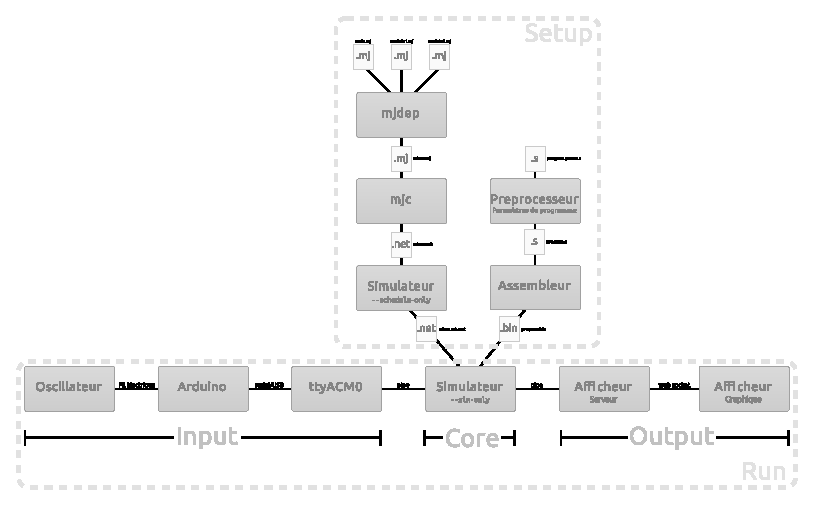
\includegraphics{organisation.eps}
\caption{\label{orga} Organisation du projet}
\end{figure}
\end{frame}

\begin{frame}
\frametitle{Vue d'ensemble}
Trois types d'information différents :
\begin{itemize}
	\item Le circuit à simuler
	\item L'état de la ROM
	\item Les entrées du circuit
\end{itemize}
\end{frame}

\begin{frame}
\frametitle{La ROM}
\begin{itemize}
	\item C'est dans la ROM qu'on va placer le programme que nous voulons exécuter par le simulateur.
		\item On donne un fichier .bin en entrée, suite de 0 et 1, qui peuvent être espacés et commentés à la suite du caractère $\#$. 
	\item	La ROM sera initialisée au lancement seulement, avec ces valeurs.
\end{itemize}
\end{frame}

\section{Fonctionnement interne}

\begin{frame}
\frametitle{La ROM}
Le simulateur peut se décomposer en plusieurs phases :
\begin{itemize}
	\item Le parseur de netlist
	\item L'optimizer, qui ordonne et simplifie les netlists
	\item Le parseur de fichier de ROM
	\item Le lecture/écriture des entrées/sorties du circuit
	\item L'initialisation, convertissant l'AST en structure plus adaptée à la simulation
	\item Le cœur du simulateur
\end{itemize}
\end{frame}



\section{Modifications}


\begin{frame}
\frametitle{Curseur de lecture}
\begin{itemize}
	\item La commande Li ne peut charger directement que de 0 à 7
	\item Il faut utiliser donc écraser tous les registres pour aller au-delà
	\item Les adresses mémoire facilement accessibles sont donc seulement de 0 à 7
	\item On crée donc un pseudo-registre \$c, pour déplacer le curseur de lecture, avec des instructions $incr$ et $decr$
	\item La RAM comporte non plus 256 mais $2^{16} = 65536$ adresses
\end{itemize}
\end{frame}


\section{Jeu d'instructions}
\begin{frame}
\frametitle{Bloc SYS}
\begin{tabular}{|c|l|l|}
  \hline
  Code & Nom & Description \\
  \hline

  \hline
  00 ** ** & \multicolumn{2}{|l|}{SYS} \\
  \hline
  00 00 10 & INCR    & Incrémente le curseur de bloc. \\
  00 00 11 & DECR    & Décrémente le curseur de bloc. \\
  \hline\hline
  00 01 00 & INPUT    & \'Ecrit l'input dans un registre donné. \\
  00 1* ** & OUTPUT x & \'Ecrit \$a0 dans la mémoire graphique\\
  00 11 11 & FLIP     & Actualise l'affichage du timer \\
\end{tabular}
\end{frame}


\begin{frame}
\frametitle{Bloc ALU}
\begin{tabular}{|c|l|l|}
  \hline
  00 ** ** & \multicolumn{2}{|l|}{ALU} \\
	  \hline
  00 00 ** & \multicolumn{2}{|l|}{Arithmétique} \\
  \hline
  01 00 00 & ADD   & \$a0 + \$a1 dans \$r0, retenue dans \$r1 \\
  01 00 01 & SUB   & \$a1 - \$a0 dans \$r0, retenue dans \$r1 \\
  01 00 10 & MULT  & \$a0 $*$ \$a1 dans \$r0 . \$r1\\
  01 00 11 & DIV   & \$a0 = \$r0 $*$ \$a1 + \$r1 \\
  \hline
  00 01 ** & \multicolumn{2}{|l|}{Logique} \\
  \hline
  01 01 00 & AND   & \$a0 AND \$a1 dans \$r0 (bit à bit) \\
  01 01 01 & OR    & \$a0 OR \$a1 dans \$r0 (bit à bit) \\
  01 01 10 & NOT   & \$r0 = NOT( \$a0 ) et \$r1 = NOT( \$a1 ) \\
  01 01 11 & SHIFT & \$r0 . \$r1 = \$a0 $*$ $2^{\text{\$a1}}$ \\
  \hline
  01 1* ** & LI x  & \$a0 = x \\
	\end{tabular}
	\end{frame}

	\begin{frame}
\frametitle{Bloc MEM}
\begin{tabular}{|c|l|l|}
\hline\hline
  10 ** ** & \multicolumn{2}{|l|}{MEM} \\
  \hline
  10 0* ** & \multicolumn{2}{|l|}{entre registres} \\
  \hline
  10 00 ij & MOVE 0ij & Déplace un \$a[i] vers un \$r[j]. \\
  10 01 ij & MOVE 1ij & Déplace un \$r[i] vers un \$a[j]. \\
  \hline
  10 1* ** & \multicolumn{2}{|l|}{avec la RAM} \\
  \hline
  10 10 ij & LOAD ij  & Charge la valeur en RAM(\$r[i]) dans \$a[j]. \\
  10 11 ij & SAVE ij  & Enregistre dans RAM(\$r[i]) la valeur \$a[j]. \\
\end{tabular}
\end{frame} 

\begin{frame}
\frametitle{Bloc JUMP}
\begin{tabular}{|c|l|l|}
  \hline\hline
  11 ** ** & \multicolumn{2}{|l|}{JUMP} \\
  \hline
  11 00 ij & JFRA ij & Ajoute \$[i][j] à l'adresse de lecture \\
  11 01 ij & JBRA ij & Retranche \$[i][j] à l'adresse de lecture \\
  11 10 ij & IIO  ij & Saute une instruction si le registre donné est $\neq 0$ \\
  11 11 0i & JAA  i  & Saut à une adresse absolue donnée par \$[i]0.\$[i]1\\
  11 11 10 & WCA     & \'Ecrit l'adresse courante dans \$a0.\$a1. \\
  11 11 11 & END      & Termine le programme. \\
  \hline
	\end{tabular}
\end{frame} 

\section{Programme de l'horloge}


\begin{frame}
\frametitle{Mémoire}
$\overline{\underbrace{\underline{|13|24|29|30|31|32|60|100|}}_{chunk 0}\underbrace{\underline{|j|m|a1|a2|h|mn|s|*|}}_{chunk 1}\underbrace{\underline{|L0|*|L2|*|*|*|*|old|}}_{chunk 2}}$
\end{frame} 


\begin{frame}
\frametitle{Difficultés}
\begin{itemize}
	\item Difficile de coder avec si peu d'instructions, mais intéressant
	\item Surtout lorsqu'il a fallu prendre en compte le nombre de jours par mois
	\item LUT dans la RAM à l'initialisation
	\item Réinitialisation de la LUT au changement d'années (pour traiter les années bisextiles)
	\end{itemize}
	\end{frame} 
	

\end{document}

